\begin{abstract}
I am proposing an emoji sequence for \textbf{NEURODIVERSITY}

\begin{figure}[h!]
\caption{\textbf{NEURODIVERSITY}}
\centering
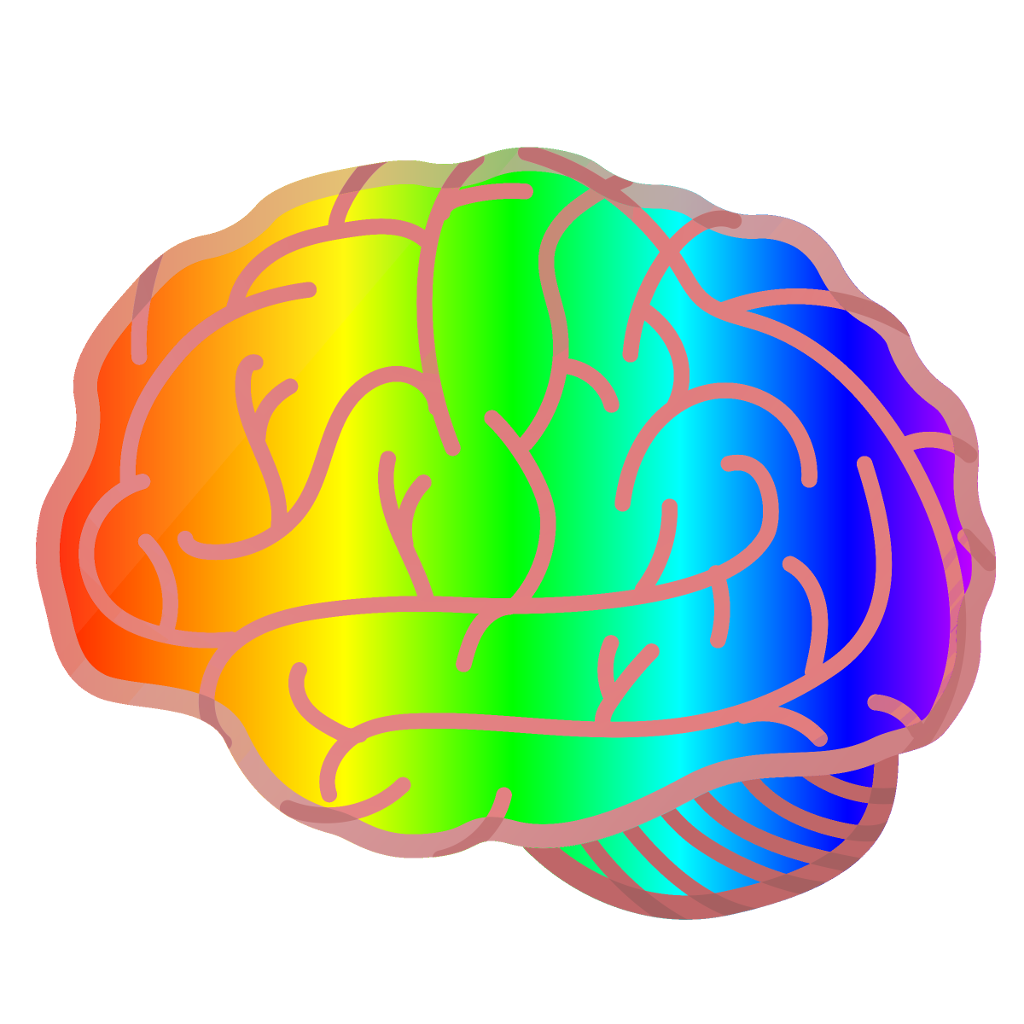
\includegraphics[width=0.333\textwidth]{neurodiversity.png}
\label{fig:neurodiversity}
\end{figure}

Autism (often referred to as Autism Spectrum Disorder) refers to a neurologically atypical brain often characterized by repetitive behaviors, differences in language processing, difficulty in social interactions, and differences in how emotions and empathy are expressed.

The center for disease control estimates that roughly 1 in 68 children is autistic. Generally boys are more likely to be diagnosed as autistic than girls, though that may be due to differences in social constructs regarding the expected behavior of boys and girls resulting is a higher percentage of autistic girls going undiagnosed.

As online social networking makes it easier for autistic individuals to find each other, our positive identity as a demographic rather than a negative identity as a disorder is starting to grow.

We believe an emoji to express our neurodiverse identity, an emoji chosen by our community, is warranted.

The primary difference between those who are autistic and those who are not is in how our brain works. A rainbow repesents the full spectrum of visible light. We believe a rainbow brain is a logical represention of the neurodiverse spectrum that makes up our community.

The unicode codepoint \texttt{U+1F9E0} is already used for a brain emoji. The unicide codepoint \texttt{U+1F308} is already used for a rainbow emoji.

The sequence of codepoints \texttt{U+1F9E0 U+200D U+1F308} could thus be an appropriate sequence to indicate a neurodiverse brain without the need for assigning a specific codepoint.
\end{abstract}
